Для сборки проекта в пакет, пригодный для использования на пользовательском компьютере был выбран компоновщик Webpack, помогающий тривиализировать сложную задачу
автоматизации построения релизного пакета приложения. Функционал Webpack упрощает процесс разработки одностраничных приложений, реализуя функционал продвинутого
разделения кода и <<горячей перезагрузки ресурсов>> (Hot Reload) для более быстрой разработки с помощью компонентной технологии пользовательского интерфейса, такой как React.
Webpack -- система сборки, которая предоставляет не только функционал компоновки модулей, но и может выполнять задачи, которые обычно выполняют специализированные task-runner системы,
такие как Gulp или Grunt. К тому же, возможности Webpack не ограничиваются обработкой JavaScript-файлов, так как он может работать с любыми видами статических ресурсов веб среды:
CSS (и языки, транслируемые в CSS), изображения, html-компоненты и, после реализации соответствующего модуля-загрузчика, любой другой тип содержимого. Webpack также поддерживает
полезную при разработки сложных веб-приложений функцию -- code splitting (разбиение кода) и dependency tree shaking (прочесывания дерева зависимостей). Большое приложение можно
разбить на подмодули и система упаковки автоматически включит их в скомпилированный ресурсный файл, в случае если он используется где-либо в системе. Все ненужные ресурсы не попадают
в результирующий исполняемый файл кроме случаев, когда это явно указано в конфигурации webpack (например, в случаях зависимости времени выполнения без соответствующей зависимости на
этапе компиляции).

Компоновщик Webpack позволяет упаковывать, компилировать, организовывать множество ресурсов и библиотек, необходимых для современного веб-проекта. Схема сборки веб проекта посредством
модулей-загрузчиков представлена на рисунке \ref{figure:domain:webpack}.

\begin{figure}[ht]
\centering
  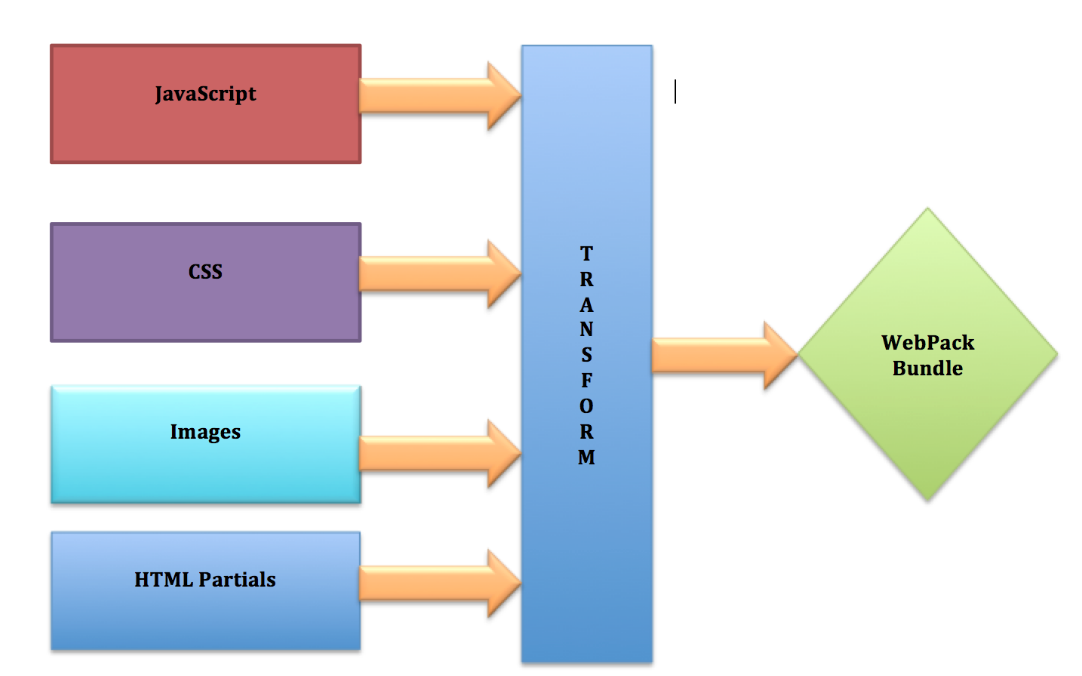
\includegraphics[scale=0.40]{webpack.png}
  \caption{Схема процесса сборки webpack}
  \label{figure:domain:webpack}
\end{figure}

Стандартные возможности Webpack включают, но не ограничиваются следующими:
\begin{itemize}
\item автоматическое построение дерева зависимостей ресурсов, в том числе зависимостей разных типов содержимого друг от друга (например, зависимости *.jsx или *.mjs файлов от каскадных таблиц
стилей *css или их прародителей, *.less/*.sass);
\item упаковка модулей, поддерживающих возможности ленивой (deferred, lazy loading) загрузки в отдельные файлы;
\item выполнение оптимизации кода, удаление ненужных элементов дерева зависимостей и минимизация получившихся исполняемых файлов;
\item поддержка функционала локального сервера ресурсов (dev server), позволяющего производить <<горячую перезагрузку ресурсов>> на странице прямо в процессе работы над проектом, что достигается
путем частичной перекомпиляции некоторых из ветвей зависимостей проекта.
\end{itemize}

Пример использования средств Webpack для организации автоматизированной сборки проекта:

Как и большинству инструментов Web-разработки, Webpack реализован на базе API Node.js -- серверной реализации JavaScript, построенной на базе движка V8. Установка Webpack производится с помощью
системы управления модулями node.js -- NPM (Node package manager). Установка производится с помощью следующей команды в терминале:

\begin{lstlisting}[language=bash, label=lst:domain:html]
npm install webpack --global
\end{lstlisting}

Данная команда установит Webpack глобально в системе (по-умолчанию установив его в директорию /usr/local/bin/npm/node\_modules), создав символические ссылки на необходимые исполняемые файлы, что
позволит запускать его из любой директории на компьютере разработчика. Далее, внутри директории проекта, был создан файл index.html с начальной разметкой:

\begin{lstlisting}[language=HTML, label=lst:domain:html]
<html lang="ru">
<head>
  <meta charset="UTF-8">
</head>
<body>
  <h2></h2>
  <script src="bundle.js"></script>
</body>
</html>
\end{lstlisting}

Важной частью этого кода является ссылка на файл bundle.js, который содержит в себе результат работы Webpack.
Первый файл определяет начальную точку приложения, в которой Webpack будет искать все зависимости. Это сработает и в том случае, если в вызываемых зависимостях 
есть свои зависимости от других модулей -- до тех пор, пока не подключатся абсолютно все необходимые модули. Таким образом, на выход получится один файл bundle.js со всем модулями.
В проекте была собрана конфигурация webpack с React.js

Точка входа в приложение:
\begin{lstlisting}[language=TypeScript, label=lst:domain:html]
const config = {
  entry: {
    app: './src/js/app.js'
  }
\end{lstlisting}

Параметры финальной упаковки:
\begin{lstlisting}[language=TypeScript, label=lst:domain:html]
  output: {
    filename: 'bundle.js',
    path: distPath
  }
\end{lstlisting}

Одной из самых важных особенностей Webpack, является возможность использовать loader. Loader по сути своей являются аналогами “задач” (tasks) в Grunt и Gulp. По существу,
они принимают содержимое файлов, а затем преобразуют его необходимым образом и включают результат преобразования в общую сборку.
Подключение React.js в бандлере:
\begin{lstlisting}[language=TypeScript, label=lst:domain:html]
 module: {
    rules: [{
      test: /\.js$/,
      exclude: [/node_modules/],
      use: [{
        loader: 'babel-loader',
        options: {
          presets: ['env', 'react']
        }
      }]
    }.
\end{lstlisting}

Для увелечения гибкости стиля был выбран язык SASS. SASS это язык похожий на HAML (весьма лаконичный шаблонизатор), но предназначенный 
для упрощения создания CSS-кода. Проще говоря, SASS это такой язык, код которого специальной ruby-программой транслируется в обычный CSS код. Синтаксис этого языка очень гибок, 
он учитывает множество мелочей, которые так желанны в CSS. 
Изменение файла конфигурации для подключение подгрузки стилей:

\begin{lstlisting}[language=TypeScript, label=lst:domain:html]
test: /\.scss$/,
      exclude: [/node_modules/],
      use: extractSass.extract({
        fallback: 'style-loader',
        use: [{
          loader: 'css-loader',
          options: {
            modules: true,
            sourceMap: true,
            importLoaders: 2,
            localIdentName: '[name]__[local]__[hash:base64:5]', // className template
            minimize: isProduction
          }
        },
          'sass-loader',
          'resolve-url-loader'
        ]
      })
\end{lstlisting}

Для работы с изображениями мы будем использовать url-loader, который является ещё одним loader для Webpack. Он берёт относительные URL 
ваших изображений и изменяет их таким образом, чтобы они корректно подключались в общем файле.
\begin{lstlisting}[language=TypeScript, label=lst:domain:html]
test: /\.(gif|png|jpe?g|svg)$/i,
      use: [{
        loader: 'file-loader',
        options: {
          name: 'images/[name][hash].[ext]'
        }
      }, {
        loader: 'image-webpack-loader',
        options: {
          mozjpeg: {
            progressive: true,
            quality: 70
          }
        }
      },
      ],}, {
      test: /\.(eot|svg|ttf|woff|woff2)$/,
      use: {
        loader: 'file-loader',
        options: {
          name: 'fonts/[name][hash].[ext]'
        }
      },
    }]
  }
\end{lstlisting}
